\documentclass[xcolor=x11names,compress]{beamer}

%% General document %%%%%%%%%%%%%%%%%%%%%%%%%%%%%%%%%%
\usepackage{graphicx}
\usepackage{tikz}
\usetikzlibrary{decorations.fractals}
%%%%%%%%%%%%%%%%%%%%%%%%%%%%%%%%%%%%%%%%%%%%%%%%%%%%%%

\makeatletter
\renewcommand\tagform@[1]{}
\makeatother


\setbeamertemplate{navigation symbols}{}

%% Beamer Layout %%%%%%%%%%%%%%%%%%%%%%%%%%%%%%%%%%
\useoutertheme[subsection=false,shadow]{miniframes}
\useinnertheme{default}
\usefonttheme{serif}
\usepackage{palatino}
\usepackage[english]{babel}
\usepackage{amsmath,amssymb,graphicx,multirow,textcomp,color}
\usepackage{epsfig,dcolumn,float,setspace}
\usepackage{setspace, graphics}
\usepackage{multirow}
\usepackage{verbatim}
\usepackage{marvosym}
\usepackage{setspace, graphics}
%\usepackage{wasysym}
\usepackage{multirow}
\usepackage{multicol}
\usepackage{verbatim}
% \usepackage{siunitx}
\usepackage{tikz}
\usetikzlibrary{shapes,backgrounds}
\usepackage{graphicx}
\usepackage{epstopdf}
\usepackage{amsmath}
\usepackage{mathrsfs}
\usepackage{lipsum}
\usepackage{bm}
\usepackage{animate}
\usepackage{algorithm}
\usepackage{caption}
\usepackage{algorithmic}
\usepackage{grffile}
\usepackage{xcolor}
 \usepackage{subfig}
 \usepackage{multirow}
\usepackage{makecell}
\usepackage{graphicx} 
\usepackage{animate}



\usepackage{float}

\usepackage{bm}

\def\T{{ \mathrm{\scriptscriptstyle T} }}
\selectlanguage{English}
\def\Put(#1,#2)#3{\leavevmode\makebox(0,0){\put(#1,#2){#3}}}


\setbeamerfont{title like}{shape=\scshape}
\setbeamerfont{frametitle}{shape=\scshape}
\definecolor{pennred}{cmyk}{0.11,.87,0.97,0.31}
\definecolor{pennblue}{cmyk}{0.95,0.81,0.13,.37}

\setbeamercolor*{lower separation line head}{bg=pennred}
\setbeamercolor*{normal text}{fg=black,bg=white}
\setbeamercolor*{alerted text}{fg=red}
\setbeamercolor*{example text}{fg=black}
\setbeamercolor*{structure}{fg=black}


\setbeamercolor*{palette tertiary}{fg=black,bg=black!10}
\setbeamercolor*{palette quaternary}{fg=black,bg=black!10}
\setbeamercolor*{palette primary}{use=structure,fg=white,bg= pennblue}
\setbeamercolor*{palette secondary}{use=structure,fg=white,bg= pennblue}
%\setbeamercolor*{palette tertiary}{use=structure,fg=white,bg= pennblue}
%\setbeamercolor*{palette quaternary}{fg=white,bg= pennred}
%\setbeamercolor*{sidebar}{use=structure,bg= pennblue}
\setbeamercolor*{palette sidebar primary}{use=structure,fg=structure.fg!10}
\setbeamercolor*{palette sidebar secondary}{fg=white}
\setbeamercolor*{palette sidebar tertiary}{use=structure,fg=structure.fg!50}
\setbeamercolor*{palette sidebar quaternary}{fg=white}
\setbeamercolor*{titlelike}{parent=palette primary}
\setbeamercolor*{separation line}{}
\setbeamercolor*{fine separation line}{}
\setbeamercolor{itemize item}{fg=pennblue}
\setbeamercolor{itemize subitem}{fg=pennblue}
\setbeamercolor{itemize subsubitem}{fg=pennblue}
\setbeamercolor{enumerate item}{fg=pennblue}

\setbeamercolor{enumerate subitem}{fg=pennblue}
\setbeamercolor{enumerate subsubitem}{fg=pennblue}
\setbeamercolor{description item}{fg=pennblue}
%\setbeamercolor{frametitle}{fg=white,bg=pennblue}
%\setbeamercolor{title in headline}{fg=pennred}


%\setbeamercolor{block}{fg=pennblue}
%\setbeamercolor{block title}{bg=pennblue,fg=pennblue}

\renewcommand{\(}{\begin{columns}}
\renewcommand{\)}{\end{columns}}
\newcommand{\<}[1]{\begin{column}{#1}}
	\renewcommand{\>}{\end{column}}

\newcommand{\barbm}[1]{ \bar{\bm{#1} }  }

\newcommand{\bi}{\begin{itemize}}
	\newcommand{\ei}{\end{itemize}}
\newcommand{\be}{\begin{enumerate}}
	\newcommand{\ee}{\end{enumerate}}

\DeclareMathOperator*{\argmax}{argmax} % thin space, limits underneath in displays
\DeclareMathOperator*{\argmin}{argmin} % thin space, limits underneath in displays


\logo{%
\makebox[.98\paperwidth]{

\includegraphics[width=2cm,height=2cm,keepaspectratio]{logos/cci_logo.jpg} 
\hfill

\includegraphics[width=3.5cm,height=3.5cm,keepaspectratio]{logos/DBEI.png}
}\vspace{-1.2cm}

}



\addtobeamertemplate{footline}{\rule{\paperwidth}{.1pt}}{\vspace{.9cm}}

\addtobeamertemplate{navigation symbols}{}{%
	
	\usebeamerfont{footline}%
	
	\usebeamercolor[fg]{footline}%
	
	\hspace{1em}%
	
	\insertframenumber/\inserttotalframenumber
}



%%%%%%%%%%%%%%%%%%%%%%%%%%%%%%%%%%%

\AtBeginSection[]
{
  \begin{frame}<beamer>
    \frametitle{Outline}
    \tableofcontents[currentsection]
  \end{frame}
}

%%%%%%%%%%%%%%%%%%%%%%%%%%%%%%%%%%%


\title{Bayesian Causal Inference in Stan}
\author[] {Arman Oganisian \\ 
\includegraphics[scale=.25]{logos/aologo.png}  }
\institute{Division of Biostatistics \\ Department of Biostatistics, Epidemiology, and Informatics \\ University of Pennsylvania}
\vspace{-100in}
\date[]{}

\begin{document}
	\maketitle

\begin{frame}
	\frametitle{Review/Tutorial paper}
	\centerline{ 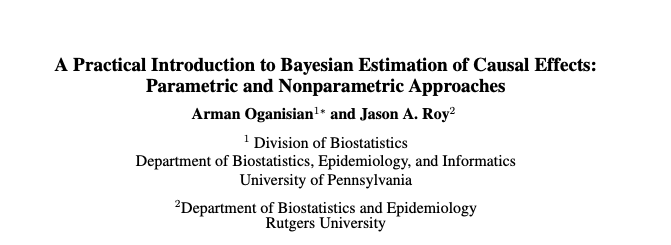
\includegraphics[scale=.5]{imgs/paper1.png}} \pause
	\Put(130,100){\color{blue}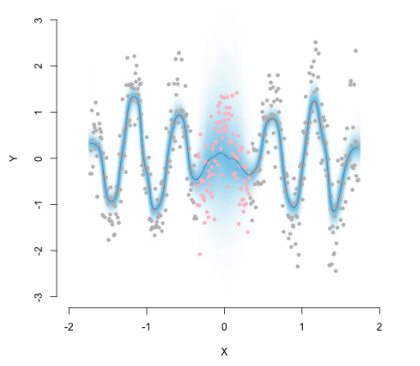
\includegraphics[scale=.3]{imgs/paper2.png}} \pause
	\Put(100,50){\color{red}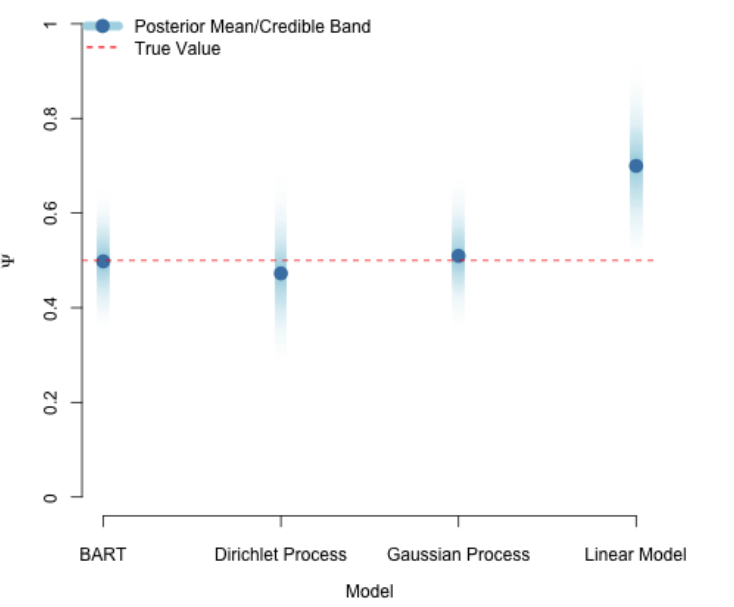
\includegraphics[scale=.2]{imgs/paper3.png}} \pause
	\Put(70,70){\color{red}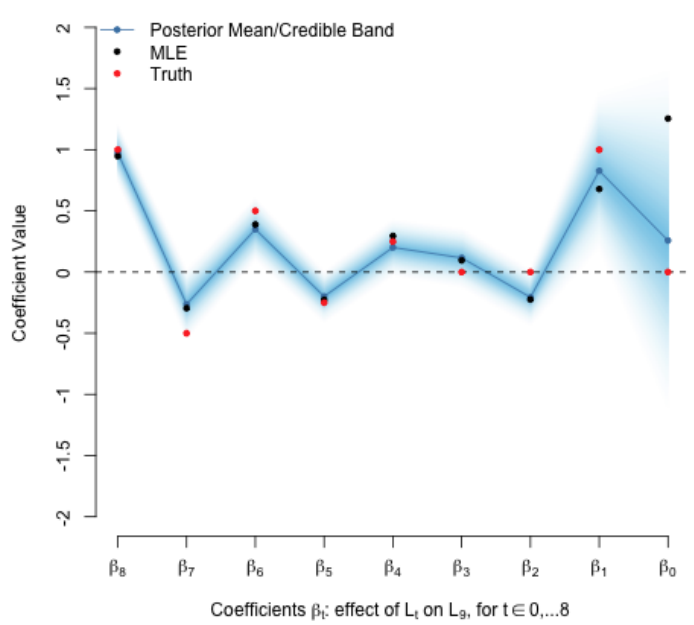
\includegraphics[scale=.2]{imgs/paper4.png}}
\end{frame}


\begin{frame}
	\frametitle{What is Causal Inference?}
	
	What \textcolor{blue}{would have happened} had everyone in the target population if ...
	\begin{itemize}
		\item ... everyone took treatment 1 versus treatment 0?  
		\item	... were vaccinated ?
		\item ... were enrolled in a job training program?
	\end{itemize}
	\pause
	\centerline{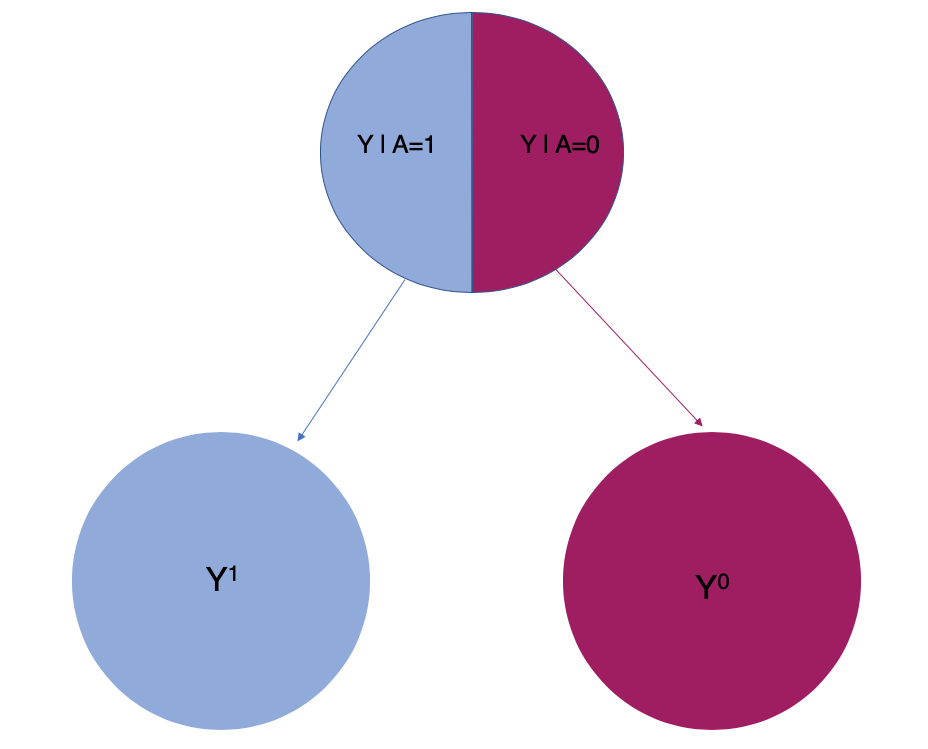
\includegraphics[scale=.15]{imgs/causal.png}}
\end{frame}

\begin{frame}
	\frametitle{Identification via the $g$-formula}
	$D = \{Y_i, A_i, L_i, V_i \}_{1:n}$. \\ 
	Define potential outcomes $Y^a$ for $a\in\{0,1\}$
	
	\pause
	$$\Psi(v) =  E[ Y^1 - Y^0 \mid V=v ]$$
	
	\pause 
	Under some \textcolor{blue}{identification assumptions}
	$$ E[Y^a \mid V=v] = \int_{\mathcal{L}} \underbrace{E[ Y\mid A=a, V=v, L ]}_{\text{Regression, $\mu(a, v, l)$ }} \underbrace{dP(L)}_{ \text{Confounder} }  $$
\end{frame}

\begin{frame}
	\frametitle{Regression Modeling}

\begin{itemize}
	\item	\textcolor{blue}{Parametric Approaches}:
	$$ \mu(A, V, L) = g^{-1}( \beta_0 +  \beta_1 A + \beta_2 V + \beta_3' L ) $$
	Need priors on $\beta$s.
	
	\item \textcolor{blue}{Nonparametric Approaches}:
	$$ \mu(A, V, L) = g^{-1}( f(A, V,  L)   ) $$	
	Need prior for $f$.
\end{itemize}
	
\end{frame}

\begin{frame}
	\frametitle{Why Bayes?}
	
	\begin{itemize}
		\item Priors can help us compute causal effects under sparsity.
		\item Avoid \textit{ad hoc} approaches.
		\item Powerful suite of nonparametric models (BART, DP, GP, etc).
		\item Probabilistic sensitivity analyses.
	\end{itemize}
\end{frame}

\begin{frame}
	\frametitle{Logistic Model For CATEs}
	Suppose $Y$ is \textcolor{blue}{binary} and $V\in\{1,2,3,4,5 \} $ (e.g., race/ethnicity)
	
	$$ Y \mid A, V, L \sim Ber \big( \mu(A, V) \big) $$
	\pause
	Specify \textcolor{blue}{logistic regression}
	$$ \mu(A, V, L) = g^{-1}( \beta_v + \beta_L' L +  \theta_v A ) $$
	with parameters $\omega = ( \beta_1\dots, \beta_5, \beta_L, \theta_1, \dots,\theta_5 )$ 
\end{frame}


\begin{frame}
	\frametitle{Prior for race effects}
	$$ \mu(A, V, L) = g^{-1}( \beta_v + \beta_L' L +  \theta_v A ) $$
	
	\begin{itemize}
	\item Consider ``partial pooling" prior: 
	\pause
	$$ \theta_v \mid \theta^* \sim N(\theta^*, \phi)  $$
	\item \textcolor{blue}{Shrinkage}: shrinkage race effects towards common effect. 
	\item \textcolor{blue}{Belief}: the race effects shouldn't be \textit{that} different. 
	\item \textcolor{blue}{Causal} intuition: small $\phi$ shrinks towards homogeneity.
	\pause
	\item Note: implies 
	$$\theta_4 - \theta_5 \sim N(0, 2\phi )$$
	As opposed to setting $\phi \approx 0$
	$$ \theta_4 - \theta_5 \sim \delta_0 $$
	\end{itemize}	
\end{frame}

\begin{frame}
	\frametitle{We have a data model...now what?}
	
	Suppose we want to compute \textcolor{blue}{Causal Odds Ratio}:
	$$ \Psi(v) = \frac{ E(Y^1 \mid v)/[1-E(Y^1 \mid v)] }{E(Y^0 \mid v)/[1-E(Y^0 \mid v)] } $$
	\pause
	Using $g$-computation, 
	$$ E(Y^a \mid v ) = \int_{\mathcal{L}} \mu(a, v, L) dP(L) $$
	
	But what about model for $P(L)$?
\end{frame}

\begin{frame}
	\frametitle{The Bayesian Bootstrap}
	
	\begin{itemize}
	 \item  \textcolor{blue}{Frequentist estimate}: $\hat P(L=l) = \sum_{i=1}^n \frac{1}{n} \cdot \delta_{L_i} (l)$
	 \pause
	 \item \textcolor{blue}{Bayesian model}: $P(L=l \mid p_{1:n}) = \sum_{i=1}^n p_i \cdot \delta_{L_i} (l)$
	 \pause
	 \begin{itemize}
	 	\item prior: 
		$$p_{1:n} \sim Dirichlet(0_n)$$
		\pause
		\item posterior: 
		$$p_{1:n} \mid L \sim Dirichlet(1_n)$$
		$$E[p_i \mid L] = 1/n $$
	 \end{itemize}
	\end{itemize}	
\end{frame}

\begin{frame}
	\frametitle{Full MCMC Inference}

	\begin{enumerate}
	\scriptsize
		\item Obtain $m^{th}$ set of posterior draws $\omega^{(m)}$ and for each $A=a$ and $V=v$
		$$  \mu^{(m)}( a, v, L_i ) = g^{-1}( \beta_v^{(m)} + \beta_L^{(m)}L_i + \theta_v^{(m)} a) $$
		
		\pause
		\item Draw Bayesian Bootstrap weights from posterior:
		$$ p_1^{(m)}, p_2^{(m)}, \dots p_n^{(m)} \sim Dirichlet(1_n) $$
		
		\pause
		\item Integrate of confounder distribution
		$$ E^{(m)}(Y^a \mid v ) = \int_{\mathcal{L}} \mu(a, v, L) dP(L) \approx \sum_{i=1}^n \mu^{(m)}( a, v, L_i ) \cdot p_i^{(m)} $$
		
		\pause
		\item Compute draw of causal odds ratio:
		$$ \Psi^{(m)} (v) = \frac{ E^{(m)}(Y^1 \mid v)/[1-E^{(m)}(Y^1 \mid v)] }{E^{(m)}(Y^0 \mid v)/[1-E^{(m)}(Y^1 \mid v)] } $$
	\end{enumerate}
\end{frame}

\begin{frame}[fragile]
	\frametitle{Implementation in Stan}
	\scriptsize
	\begin{verbatim}
	
generated quantities {
vector[N] bb_weights = dirichlet_rng( rep_vector( 1, N) ) ;

...

for( v in 1:Pv ){
  for(i in 1:N){
    cond_mean_y1[i] = inv_logit( L[i]*beta_L + beta_v[v] + theta[v]);
    cond_mean_y0[i] = inv_logit( L[i]*beta_L + beta_v[v] );
  }
  marg_mean_y1 = bb_weights' * cond_mean_y1 ;
  marg_mean_y0 = bb_weights' * cond_mean_y0 ;
	
  odds_1 = marg_mean_y1/(1 - marg_mean_y1);
  odds_0 = marg_mean_y0/(1 - marg_mean_y0);
  odds_ratio[v] = odds_1 / odds_0;
}
...
}

	\end{verbatim}
\end{frame}

\begin{frame}
	\frametitle{Synthetic Example}
	\centerline{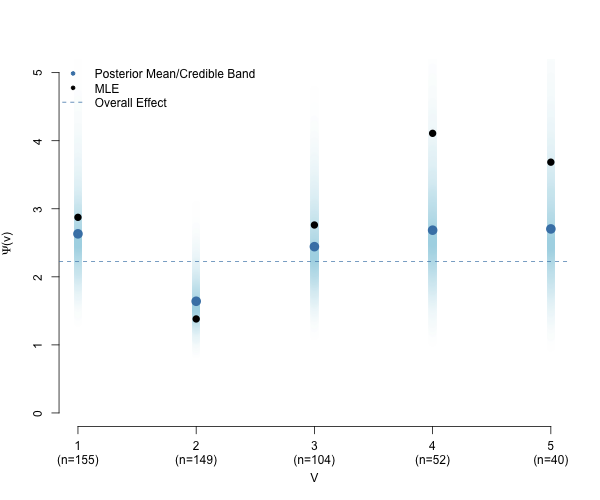
\includegraphics[scale=.4]{code/ppooling_plot.png}}
\end{frame}


\begin{frame}
	\frametitle{Sensitivity Analysis}
	
	Identification requires \textcolor{blue}{conditional ignorability}
	$$ Y^a \perp A \mid L, V=v $$

	But, what if ignorability is violated?
	$$ E[Y^a \mid A=1, L, v] \neq E[Y^a \mid A=0, L, v]  $$
\end{frame}

\begin{frame}
	\frametitle{Consequence of Violation}
	
	Define, 	
	$$\Delta^a(L)  = E[Y^a \mid A=1, L, v] - E[Y^a \mid A=0, L, v] $$
	
	\pause
	$$\int \mu(1,v, L) - \mu(0, v, L) \ dP(L)  = E[Y^1 - Y^0 \mid v ] + \xi$$
	
	Estimate of \textcolor{blue}{risk difference} is biased by $\xi$.
		
\end{frame}


\begin{frame}
	\frametitle{Form of Violation}
	Trade-offs involved in sensitivity analyses
	$$ \xi = \int \Delta^1(L)(1- \pi(L)) + \Delta^0(L) \pi(L)  \ dP(L) $$
	Simplify $ \Delta := \Delta^1 = \Delta^0$ and $ \Delta \perp L$. Then, 
	
	$$ \xi = \Delta $$
	
	Now we can specify priors over $\Delta$.
\end{frame}

\begin{frame}
	\frametitle{Priors over bias}
	Note that $-1 < E[Y^1 - Y^0 \mid v ] < 1$ and recall:
	$$\Delta  = E[Y^a \mid A=1, L, v] - E[Y^a \mid A=0, L, v] $$
	
	\begin{itemize}
		\pause
		\item Treated patients \textcolor{blue}{systematically worse}:
		$$ \Delta \sim U(0, 1) $$
		
		\pause
		\item Treated patients \textcolor{blue}{systematically better}:
		$$ \Delta \sim U(-1, 0) $$
		
		\pause
		\item Biased with \textcolor{blue}{uncertain direction}:
		$$ \Delta \sim U(-1,1) $$		
	\end{itemize}
\end{frame}

\begin{frame}
	\frametitle{Modified MCMC Inference}

	In Step 3 at $m^{th}$ iteration: \\


	Draw $\Delta^{(m)}$ from the prior and compute, 
	
	$$ E^{(m)}(Y^a \mid v ) =  \Big\{ \sum_{i=1}^n \mu^{(m)}( a, v, L_i ) \cdot p_i^{(m)} \Big\} - \Delta^{(m)} $$

\end{frame}

\begin{frame}
	\frametitle{Implementation in Stan}

	\begin{itemize}
		\item Could specify prior for $\Delta$ in ``model" block. Manipulate in ``generated quantities".
		\item Could draw $\Delta$ from specified distribution in ``generated quantities" block.
	\end{itemize}
\end{frame}

\begin{frame}
	\frametitle{Some Resources}

	\begin{itemize}
		\item A Practical Introduction to Bayesian Estimation of Causal Effects: Parametric and Nonparametric Approaches
		\url{https://arxiv.org/pdf/2004.07375.pdf}
		\item Companion GitHub repo for paper:
		\url{https://github.com/stablemarkets/intro_bayesian_causal}
		\item GitHub Repo for this talk:
		\url{https://github.com/stablemarkets/StanCon2020_BayesCausal}
	\end{itemize}
\end{frame}

\begin{frame}
	\frametitle{Thank you!}

\end{frame}

\end{document}
			
			
